%% ============================================================
%%  UKF on Lie Groups for GNSS/INS Integration
%%  Full Technical Documentation
%% ============================================================
\documentclass[11pt,a4paper]{article}

%% --- Packages ---
\usepackage[T1]{fontenc}
\usepackage[utf8]{inputenc}
\usepackage[english]{babel}
\usepackage{lmodern}
\usepackage{microtype}
\usepackage{geometry}
\geometry{margin=2.5cm}

%% Math
\usepackage{amsmath,amssymb,amsthm,bm}
\usepackage{mathtools}
\usepackage{physics}
\usepackage{siunitx}

%% Figures & TikZ
\usepackage{graphicx}
\usepackage{tikz}
\usepackage{pgfplots}
\pgfplotsset{compat=1.18}
\usetikzlibrary{
  arrows.meta, shapes.geometric, shapes.multipart,
  positioning, fit, backgrounds, calc,
  decorations.pathreplacing, decorations.markings,
  matrix, chains, shadows.blur
}

%% Tables
\usepackage{booktabs}
\usepackage{array}
\usepackage{multirow}

%% Code listings
\usepackage{listings}
\usepackage{xcolor}
\lstset{
  language=Matlab,
  basicstyle=\ttfamily\small,
  keywordstyle=\color{blue}\bfseries,
  commentstyle=\color{gray}\itshape,
  stringstyle=\color{orange},
  numbers=left, numberstyle=\tiny\color{gray},
  breaklines=true, frame=single, backgroundcolor=\color{gray!8}
}

%% Colors
\definecolor{lieblue}{RGB}{25,84,163}
\definecolor{liegray}{RGB}{240,242,246}
\definecolor{lieaccent}{RGB}{230,80,30}
\definecolor{liegreen}{RGB}{30,140,80}
\definecolor{lieyellow}{RGB}{210,160,20}

%% Hyperref
\usepackage{hyperref}
\hypersetup{colorlinks=true,linkcolor=lieblue,citecolor=liegreen,urlcolor=lieaccent}

%% Theorem environments
\theoremstyle{definition}
\newtheorem{definition}{Definition}[section]
\newtheorem{remark}{Remark}[section]
\theoremstyle{plain}
\newtheorem{theorem}{Theorem}[section]
\newtheorem{proposition}{Proposition}[section]

%% Custom macros
\newcommand{\SO}{\mathrm{SO}(3)}
\newcommand{\so}{\mathfrak{so}(3)}
\newcommand{\Exp}{\mathrm{Exp}}
\newcommand{\Log}{\mathrm{Log}}
\newcommand{\Ad}{\mathrm{Ad}}
\newcommand{\Ceb}{\mathbf{C}_{eb}}
\newcommand{\veb}{\mathbf{v}_{eb}^e}
\newcommand{\peb}{\mathbf{p}_{eb}^e}
\newcommand{\ba}{\mathbf{b}_a}
\newcommand{\bg}{\mathbf{b}_g}
\newcommand{\fib}{\mathbf{f}_{ib}^b}
\newcommand{\wib}{\bm{\omega}_{ib}^b}
\newcommand{\bX}{\mathbf{X}}
\newcommand{\bP}{\mathbf{P}}
\newcommand{\bQ}{\mathbf{Q}}
\newcommand{\bR}{\mathbf{R}}
\newcommand{\bK}{\mathbf{K}}
\newcommand{\beps}{\bm{\varepsilon}}
\newcommand{\skewb}[1]{[#1]_\times}

%% Header
\usepackage{fancyhdr}
\pagestyle{fancy}
\fancyhf{}
\fancyhead[L]{\small\textcolor{lieblue}{\textbf{UKF on Lie Groups}}}
\fancyhead[R]{\small\textcolor{lieblue}{GNSS/INS Integration}}
\fancyfoot[C]{\thepage}
\renewcommand{\headrulewidth}{0.5pt}

\begin{document}

%% ---- Title Page ----
\begin{titlepage}
\begin{tikzpicture}[remember picture, overlay]
  \fill[lieblue!90!black] (current page.north west) rectangle
        ([yshift=-6cm]current page.north east);
  \fill[lieblue!40!white, opacity=0.4]
        ([yshift=-4cm]current page.north west) --
        ([yshift=-6cm]current page.north east) --
        ([yshift=-4.5cm]current page.north east) -- cycle;
  \fill[lieaccent] (current page.south west) rectangle
        ([yshift=1.2cm]current page.south east);
\end{tikzpicture}
\vspace*{1.5cm}
\begin{center}
  {\Huge\bfseries\textcolor{lieblue!90!black}
    {Unscented Kalman Filter}\\[0.3em]
    \textcolor{lieblue}
    {on Lie Groups}\\[0.6em]}
  {\LARGE\textcolor{lieblue!60!black}
    {for GNSS/INS Tightly-Coupled Navigation}}
  \vspace{1.5cm}
  \rule{0.7\textwidth}{1.5pt}
  \vspace{0.5cm}
  {\large Technical Documentation\\[0.3em]
   Implementation Reference Manual}
  \vspace{2cm}
  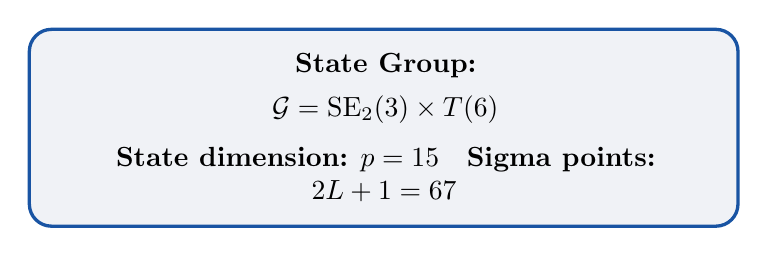
\begin{tikzpicture}
    \node[draw=lieblue, fill=liegray, rounded corners=8pt,
          minimum width=9cm, minimum height=2.5cm,
          line width=1.2pt] at (0,0) {
      \begin{minipage}{8cm}\centering
        \textbf{State Group:}\\[4pt]
        $\mathcal{G} = \mathrm{SE}_2(3) \times T(6)$\\[6pt]
        \textbf{State dimension:} $p = 15$\quad
        \textbf{Sigma points:} $2L+1 = 67$
      \end{minipage}
    };
  \end{tikzpicture}
  \vspace{3cm}
  {\large \textit{Scientific Initiation Project}\\[0.6em]
   \today}
\end{center}
\end{titlepage}

\tableofcontents
\newpage

\section{Introduction}

Inertial Navigation Systems (INS) fused with Global Navigation Satellite Systems (GNSS)
constitute the backbone of modern navigation.
Classical Kalman filtering approaches parametrise the vehicle attitude with Euler angles or
quaternions and propagate the covariance in $\mathbb{R}^n$, ignoring the underlying
non-Euclidean geometry of the state space.
This leads to linearisation errors and singularities near gimbal-lock.

The \emph{UKF on Lie Groups} (UKF-Lie) addresses this by working directly on a
matrix Lie group $\mathcal{G}$, using the group exponential and logarithm to
map between the manifold and its tangent space (the Lie algebra) only when
computing means and covariances.
The sigma-point propagation itself remains entirely on the group, preserving
the rotation-matrix structure at every step.

\subsection{Notation}

\begin{table}[h!]
\centering
\caption{Symbol notation.}
\label{tab:notation}
\renewcommand{\arraystretch}{1.4}
\begin{tabular}{@{}lll@{}}
\toprule
Symbol & Dimension & Description \\
\midrule
$\Ceb \in \SO$ & $3\times 3$ & Rotation matrix: body $\to$ ECEF \\
$\veb \in \mathbb{R}^3$ & $3\times 1$ & Velocity of body in ECEF frame \\
$\peb \in \mathbb{R}^3$ & $3\times 1$ & Position of body in ECEF frame \\
$\ba \in \mathbb{R}^3$ & $3\times 1$ & Accelerometer bias \\
$\bg \in \mathbb{R}^3$ & $3\times 1$ & Gyroscope bias \\
$\fib \in \mathbb{R}^3$ & $3\times 1$ & Specific force (accelerometer measurement) \\
$\wib \in \mathbb{R}^3$ & $3\times 1$ & Angular rate (gyroscope measurement) \\
$\bX \in \mathcal{G}$ & $13\times 13$ & Full navigation state on the Lie group \\
$\bP \in \mathbb{R}^{p\times p}$ & $15\times 15$ & Error covariance in the Lie algebra \\
$\bQ$ & $15\times 15$ & Process noise covariance \\
$\bR$ & $3\times 3$ & Measurement noise covariance \\
$L = 2p+q$ & $33$ & Augmented state dimension \\
$\alpha,\beta,\kappa$ & scalars & UT scaling parameters \\
$\lambda$ & scalar & $\alpha^2(L+\kappa)-L$ \\
\bottomrule
\end{tabular}
\end{table}

\section{Lie Group Fundamentals}

\subsection{The Special Orthogonal Group SO(3)}

\begin{definition}[$\SO$]
The special orthogonal group:
\[
  \SO = \{\mathbf{C}\in\mathbb{R}^{3\times 3} \mid \mathbf{C}^\top\mathbf{C} = \mathbf{I},\;
         \det(\mathbf{C})=+1\}.
\]
\end{definition}

For $\bm{\phi} = \phi\,\mathbf{a}$, the hat operator: $\skewb{\bm\phi}_{ij} = -\epsilon_{ijk}\phi_k$.

\textbf{Exponential map} (Rodrigues formula):
\[
  \Exp(\bm\phi) = \mathbf{I} + \frac{\sin\phi}{\phi}\skewb{\bm\phi}
                + \frac{1-\cos\phi}{\phi^2}\skewb{\bm\phi}^2.
\]

\textbf{Logarithmic map}:
\[
  \phi = \arccos\!\left(\tfrac{\tr(\mathbf{C})-1}{2}\right), \qquad
  \mathbf{a} = \frac{1}{2\sin\phi}\left(\mathbf{C}-\mathbf{C}^\top\right)^\vee, \qquad
  \Log(\mathbf{C}) = \phi\,\mathbf{a}.
\]

\subsection{The Extended Pose Group SE2(3)}

\begin{definition}[$\mathrm{SE}_2(3)$]
\[
  \mathrm{SE}_2(3) = \left\{
    \begin{pmatrix}\mathbf{C} & \mathbf{v} & \mathbf{p}\\
                   \mathbf{0}_{2\times 3} & \mathbf{I}_2\end{pmatrix}
    \in\mathbb{R}^{5\times5}
    \;\Big|\; \mathbf{C}\in\SO,\;
              \mathbf{v},\mathbf{p}\in\mathbb{R}^3 \right\}.
\]
\end{definition}

\textbf{Exponential map} (\texttt{exp\_multiSE3.m}):
\[
  \Exp(\xi) = \mathbf{I}_{5} + \Xi +
              \frac{1-\cos\theta}{\theta^2}\,\Xi^2 +
              \frac{\theta-\sin\theta}{\theta^3}\,\Xi^3,
  \quad \theta = \|\bm\phi\|.
\]

\textbf{Logarithmic map} (\texttt{log\_multiSE3.m}):
\[
  \Log(\mathbf{X}) = \begin{pmatrix} \phi\,\mathbf{a} \\
                     \mathbf{J}^{-1}(\phi)\,\mathbf{r}_v \\
                     \mathbf{J}^{-1}(\phi)\,\mathbf{r}_p
                     \end{pmatrix}\!, \qquad
  \mathbf{J}^{-1}(\phi) = \frac{\phi}{2}\cot\frac{\phi}{2}\,\mathbf{I}
            + \left(1-\frac{\phi}{2}\cot\frac{\phi}{2}\right)\mathbf{a}\mathbf{a}^\top
            - \frac{\phi}{2}\skewb{\mathbf{a}}.
\]

\subsection{Full State Group}

The $13\times13$ block-diagonal navigation state:
\[
  \bX = \mathrm{blkdiag}\!\left(
    \begin{pmatrix}\Ceb & \veb & \peb\\\mathbf{0}&\mathbf{I}\end{pmatrix},\;
    \begin{pmatrix}\mathbf{I} & \ba\\\mathbf{0} & 1\end{pmatrix},\;
    \begin{pmatrix}\mathbf{I} & \bg\\\mathbf{0} & 1\end{pmatrix}
  \right)\!\in\mathbb{R}^{13\times13}.
\]

Adjoint map (\texttt{Ad\_G.m}):
\[
  \Ad_{\bX} =
  \begin{pmatrix}
    \Ceb & \mathbf{0} & \mathbf{0} \\
    \skewb{\veb}\Ceb & \Ceb & \mathbf{0} \\
    \skewb{\peb}\Ceb & \mathbf{0} & \Ceb
  \end{pmatrix} \oplus \mathbf{I}_6.
\]

\section{Navigation Model}

\subsection{Reference Frames}

\begin{figure}[h!]
\centering
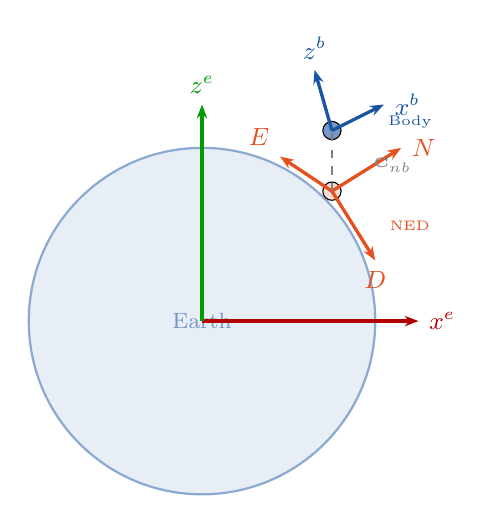
\begin{tikzpicture}[scale=1.1,
  frame/.style={-{Stealth[length=5pt]}, very thick},
  lbl/.style={font=\small\bfseries}
]
\draw[fill=lieblue!10, draw=lieblue!50, thick] (0,0) ellipse (2cm and 2cm);
\node[lieblue!60, font=\footnotesize] at (0,0) {Earth};
\draw[frame, red!70!black] (0,0) -- (2.5,0) node[lbl,right]{$x^e$};
\draw[frame, green!60!black] (0,0) -- (0,2.5) node[lbl,above]{$z^e$};
\coordinate (ned) at (1.5,1.5);
\draw[fill=lieaccent!20] (ned) circle (3pt);
\draw[frame, lieaccent] (ned) -- ++(0.8,0.5) node[lbl,right]{$N$};
\draw[frame, lieaccent] (ned) -- ++(0.5,-0.8) node[lbl,below]{$D$};
\draw[frame, lieaccent] (ned) -- ++(-0.6,0.4) node[lbl,above left]{$E$};
\coordinate (body) at (1.5,2.2);
\draw[fill=lieblue!60] (body) circle (3pt);
\draw[frame, lieblue] (body) -- ++(0.6,0.3) node[lbl,right]{$x^b$};
\draw[frame, lieblue] (body) -- ++(-0.2,0.7) node[lbl,above]{$z^b$};
\node[font=\tiny,lieaccent] at (2.4,1.1) {NED};
\node[font=\tiny,lieblue] at (2.4,2.3) {Body};
\draw[dashed,gray] (ned) -- (body);
\node[gray, font=\tiny] at (2.2,1.8) {$\mathbf{C}_{nb}$};
\end{tikzpicture}
\caption{Reference frames: ECEF (red/green), local NED (orange), and body frame (blue).}
\label{fig:frames}
\end{figure}

Rotation NED to ECEF (\texttt{DCM\_en.m}):
\[
  \mathbf{C}_{en}(\lambda,\ell) =
  \begin{pmatrix}
    -\sin\lambda\cos\ell & -\sin\ell & -\cos\lambda\cos\ell \\
    -\sin\lambda\sin\ell &  \cos\ell & -\cos\lambda\sin\ell \\
     \cos\lambda         &  0        & -\sin\lambda
  \end{pmatrix}\!.
\]

WGS-84 gravity (\texttt{gravityModel.m}):
\[
  g(\lambda) = \frac{g_0\,(1 + g_1\sin^2\!\lambda)}
                    {\sqrt{1 - e^2\sin^2\!\lambda}},
  \quad g_0 = 9.7803267714\,\mathrm{m/s^2},\;\;
  g_1 = 1.93185\times10^{-3},\;\;
  e = 0.0818.
\]

\subsection{Process Model}

Left-invariant continuous-time dynamics (\texttt{Omega.m}):
\[
  \dot{\mathbf{X}} = \mathbf{X}\,\Omega^\wedge, \qquad
  \Omega =
  \begin{pmatrix}
    \wib - \bg \\
    \mathbf{C}_{be}(g_n\fib - \ba) + \mathbf{C}_{be}\mathbf{g}^e \\
    \mathbf{C}_{be}\veb \\
    \mathbf{0}_6
  \end{pmatrix}\!\in\mathbb{R}^{15}.
\]

Discrete integration:
\[
  \bX_{k} = \bX_{k-1}\,\Exp(\Omega_{k-1}\,\Delta t + \bm{q}_{k-1}),
  \quad \bm{q}_{k-1}\sim\mathcal{N}(\mathbf{0},\bQ).
\]

\subsection{Measurement Model}

GNSS position with lever arm compensation:
\[
  h(\bX) = \peb + \Ceb\,\bm\ell_b \in\mathbb{R}^3,
  \qquad
  Y = \begin{pmatrix}\mathbf{I}_3 & h(\bX) \\ \mathbf{0} & 1\end{pmatrix}\!\in T(3).
\]

Innovation (since $T(3)$ is a vector group):
$\bm\delta = \mathbf{y}_k - h(\bX)$.

\section{Unscented Kalman Filter on Lie Groups}

\subsection{Augmented State}

\[
  \bm\eta = (\bm\varepsilon^\top, \mathbf{q}^\top, \mathbf{r}^\top)^\top \in\mathbb{R}^L,
  \quad L = 2p + q = 33,
  \qquad
  \mathbf{P}_\eta = \mathrm{blkdiag}(\bP,\bQ,\bR).
\]

Weights ($\alpha=0.014$, $\beta=2$, $\kappa=0$, $\lambda=\alpha^2(L+\kappa)-L$):
\[
  W_m^{(0)} = \frac{\lambda}{L+\lambda}, \quad
  W_c^{(0)} = \frac{\lambda}{L+\lambda} + (1-\alpha^2+\beta), \quad
  W_m^{(i)} = W_c^{(i)} = \frac{1}{2(L+\lambda)}, \; i\geq1.
\]

\subsection{Sigma Points (\texttt{SigmaPointsLie.m})}

$\mathbf{S} = \mathrm{chol}(\mathbf{P}_\eta)^\top$ (lower triangular):
\[
  \bm\xi^{(0)} = \mathbf{0}_L, \quad
  \bm\xi^{(i)} = +\sqrt{L+\lambda}\,\mathbf{S}_{:,i}, \quad
  \bm\xi^{(i+L)} = -\sqrt{L+\lambda}\,\mathbf{S}_{:,i}, \quad i=1,\ldots,L.
\]

\subsection{Prediction (\texttt{prediction\_UKF\_Lie.m})}

\begin{align}
  \mathcal{X}_{k-1}^{(i)} &= \bX_{k-1}\,\Exp(\bm{e}^{(i)}) \tag{lift}\\
  \mathcal{X}_{k|k-1}^{(i)} &= \mathcal{X}_{k-1}^{(i)}\,\Exp(\Omega^{(i)}\Delta t + \mathbf{q}^{(i)}) \tag{propagate}\\
  \bar{\mathbf{X}}_k &= \text{Frechet mean}\{\mathcal{X}_{k|k-1}^{(i)}, W_m^{(i)}\} \tag{mean}\\
  \bm\varepsilon^{(i)} &= \Log(\bar{\mathbf{X}}_k^{-1}\mathcal{X}_{k|k-1}^{(i)}) \tag{algebra errors}\\
  \bP_{k|k-1} &= \sum_i W_c^{(i)}\bm\varepsilon^{(i)}(\bm\varepsilon^{(i)})^\top + \bQ \tag{covariance}
\end{align}

Frechet mean iteration (\texttt{media\_nula\_g.m}):
\[
  \bar{\mathbf{X}}^{(j+1)} = \bar{\mathbf{X}}^{(j)}\,
  \Exp\!\!\left(\alpha^2\sum_{i} W_m^{(i)}\Log\!\left((\bar{\mathbf{X}}^{(j)})^{-1}
  \mathcal{X}^{(i)}\right)\right)
\]
until $\|\bm\sigma^{(j)}\|<10^{-3}$ (max 30 iterations).

\subsection{Update (\texttt{Update\_UKF\_Lie.m})}

\begin{align}
  \mathcal{Y}^{(i)} &= \begin{pmatrix}\mathbf{I} & \mathbf{p}^{(i)}+\mathbf{C}^{(i)}\bm\ell_b+\mathbf{r}^{(i)}\\\mathbf{0}&1\end{pmatrix} \tag{meas sigma pts}\\
  \bar{\mathbf{y}} &= \alpha^2\sum_i W_m^{(i)}\mathbf{y}^{(i)} \tag{predicted mean}\\
  \mathbf{P}_{hh} &= \sum_i W_c^{(i)}\bm\delta^{(i)}(\bm\delta^{(i)})^\top + \bR \tag{innovation cov}\\
  \mathbf{P}_{gh} &= \sum_i W_c^{(i)}\bm\varepsilon^{(i)}(\bm\delta^{(i)})^\top \tag{cross cov}\\
  \bK &= \mathbf{P}_{gh}\mathbf{P}_{hh}^{-1} \tag{Kalman gain}\\
  \bX_{k|k} &= \bar{\mathbf{X}}_k\,\Exp(\bK(\mathbf{y}_k-\bar{\mathbf{y}})) \tag{state update}\\
  \bP_{k|k} &= \bP_{k|k-1} - \bK\,\mathbf{P}_{gh}^\top \tag{covariance update}
\end{align}

\section{Workflow and Pipeline}

\subsection{High-Level Architecture}

\begin{figure}[!ht]
\centering
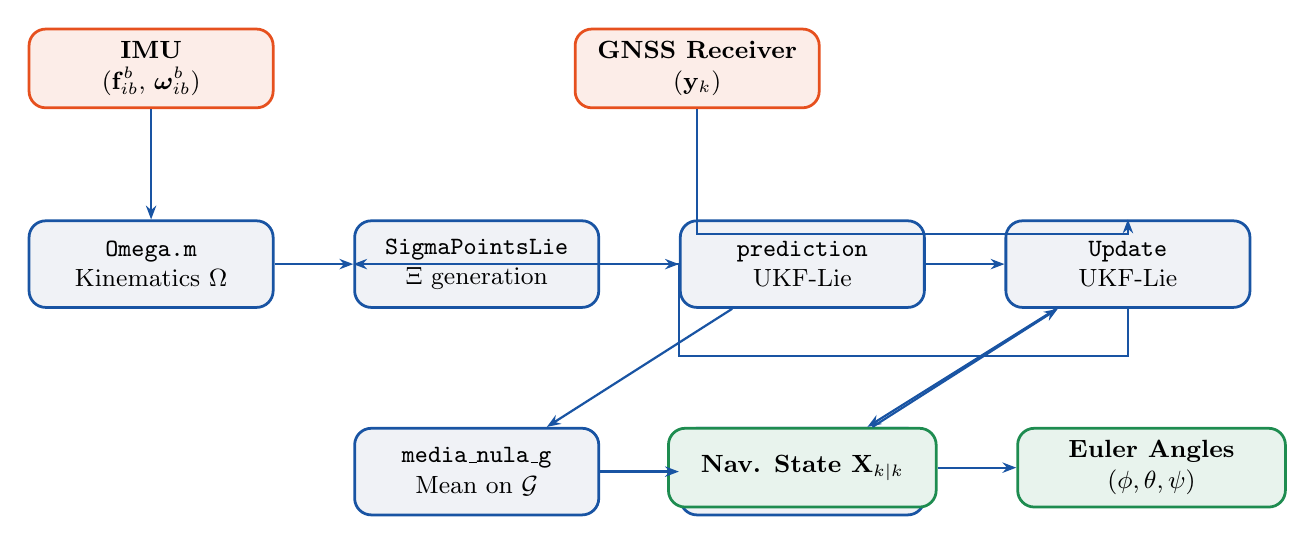
\begin{tikzpicture}[
  node distance=0.8cm and 1.2cm,
  box/.style={draw=lieblue, fill=liegray, rounded corners=6pt,
              minimum width=3.1cm, minimum height=1.1cm,
              align=center, font=\small, line width=1.0pt},
  sensor/.style={draw=lieaccent, fill=lieaccent!10, rounded corners=6pt,
                 minimum width=3.1cm, minimum height=1.0cm,
                 align=center, font=\small\bfseries, line width=1.0pt},
  output/.style={draw=liegreen, fill=liegreen!10, rounded corners=6pt,
                 minimum width=3.4cm, minimum height=1.0cm,
                 align=center, font=\small\bfseries, line width=1.0pt},
  arr/.style={-{Stealth[length=5pt]}, thick, lieblue}
]
\node[sensor] (imu) {IMU\\$(\fib,\,\wib)$};
\node[sensor, right=3.8cm of imu] (gps) {GNSS Receiver\\$(\mathbf{y}_k)$};
\node[box, below=1.4cm of imu] (omega) {\texttt{Omega.m}\\Kinematics $\Omega$};
\node[box, right=1.0cm of omega] (sigpred) {\texttt{SigmaPointsLie}\\$\Xi$ generation};
\node[box, right=1.0cm of sigpred] (pred) {\texttt{prediction}\\UKF-Lie};
\node[box, right=1.0cm of pred] (upd) {\texttt{Update}\\UKF-Lie};
\node[box, below=1.5cm of sigpred] (mean) {\texttt{media\_nula\_g}\\Mean on $\mathcal{G}$};
\node[box, right=1.0cm of mean] (cov) {\texttt{covariancias}\\$\mathbf{P}_{gh},\mathbf{P}_{hh}$};
\node[output, below=1.5cm of pred] (state) {Nav. State $\bX_{k|k}$};
\node[output, right=1.0cm of state] (euler) {Euler Angles\\$(\phi,\theta,\psi)$};
\draw[arr] (imu) -- (omega);
\draw[arr] (omega) -- (sigpred);
\draw[arr] (sigpred) -- (pred);
\draw[arr] (pred) -- (upd);
\draw[arr] (gps) -- ++(0,-2.1) -| (upd);
\draw[arr] (pred) -- (mean);
\draw[arr] (mean) -- (cov);
\draw[arr] (cov) -- (upd);
\draw[arr] (upd) -- (state);
\draw[arr] (state) -- (euler);
% feedback loop routed below all bottom-row nodes
\draw[arr] (upd.south) -- ++(0,-0.6)
           -- ++(-5.7,0) |- (sigpred.west);
\end{tikzpicture}
\caption{High-level architecture and data flow of the UKF-Lie system.}
\label{fig:architecture}
\end{figure}

\subsection{Prediction Flowchart}

\begin{figure}[!ht]
\centering
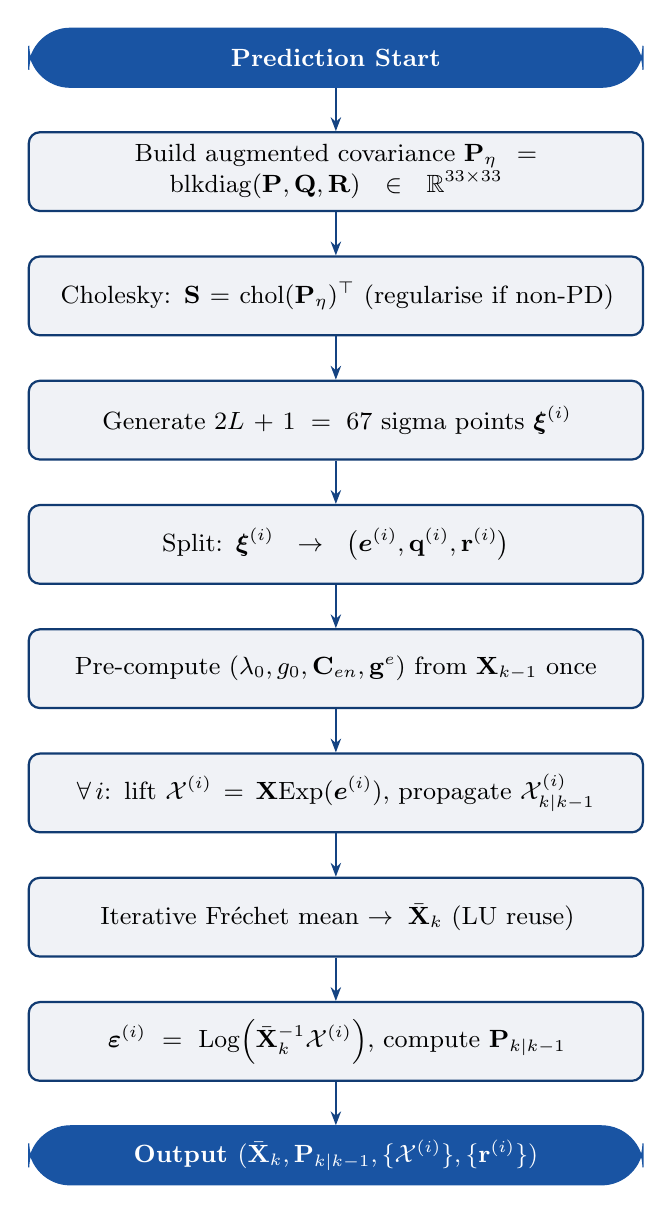
\begin{tikzpicture}[
  node distance=0.55cm,
  start/.style={draw=lieblue, fill=lieblue, text=white, rounded corners=15pt,
                minimum width=7.8cm, minimum height=0.75cm, font=\small\bfseries},
  flowstep/.style={draw=lieblue!70!black, fill=liegray, rounded corners=4pt,
               minimum width=7.8cm, minimum height=1.0cm,
               text width=7.4cm,
               align=center, font=\small, line width=0.8pt},
  arr/.style={-{Stealth[length=5pt]}, thick, lieblue!80!black}
]
\node[start] (s0) {Prediction Start};
\node[flowstep, below=0.55cm of s0] (s1)
  {Build augmented covariance
   $\mathbf{P}_\eta=\mathrm{blkdiag}(\bP,\bQ,\bR)\in\mathbb{R}^{33\times33}$};
\node[flowstep, below=0.55cm of s1] (s2)
  {Cholesky: $\mathbf{S}=\mathrm{chol}(\mathbf{P}_\eta)^\top$ (regularise if non-PD)};
\node[flowstep, below=0.55cm of s2] (s3)
  {Generate $2L+1=67$ sigma points $\bm\xi^{(i)}$};
\node[flowstep, below=0.55cm of s3] (s4)
  {Split: $\bm\xi^{(i)}\to\bigl(\bm{e}^{(i)},\mathbf{q}^{(i)},\mathbf{r}^{(i)}\bigr)$};
\node[flowstep, below=0.55cm of s4] (s5)
  {Pre-compute $(\lambda_0,g_0,\mathbf{C}_{en},\mathbf{g}^e)$ from $\bX_{k-1}$ once};
\node[flowstep, below=0.55cm of s5] (s6)
  {$\forall\,i$: lift $\mathcal{X}^{(i)}=\bX\Exp(\bm{e}^{(i)})$,
   propagate $\mathcal{X}_{k|k-1}^{(i)}$};
\node[flowstep, below=0.55cm of s6] (s7)
  {Iterative Fréchet mean $\to\bar{\mathbf{X}}_k$ (LU reuse)};
\node[flowstep, below=0.55cm of s7] (s8)
  {$\bm\varepsilon^{(i)}=\Log\!\left(\bar{\mathbf{X}}_k^{-1}\mathcal{X}^{(i)}\right)$,
   compute $\bP_{k|k-1}$};
\node[start, below=0.55cm of s8] (s9)
  {Output $(\bar{\mathbf{X}}_k,\bP_{k|k-1},\{\mathcal{X}^{(i)}\},\{\mathbf{r}^{(i)}\})$};
\foreach \a/\b in {s0/s1,s1/s2,s2/s3,s3/s4,s4/s5,s5/s6,s6/s7,s7/s8,s8/s9}
  \draw[arr] (\a) -- (\b);
\end{tikzpicture}
\caption{Prediction step flowchart.}
\label{fig:pred_flow}
\end{figure}

\subsection{Update Flowchart}

\begin{figure}[!ht]
\centering
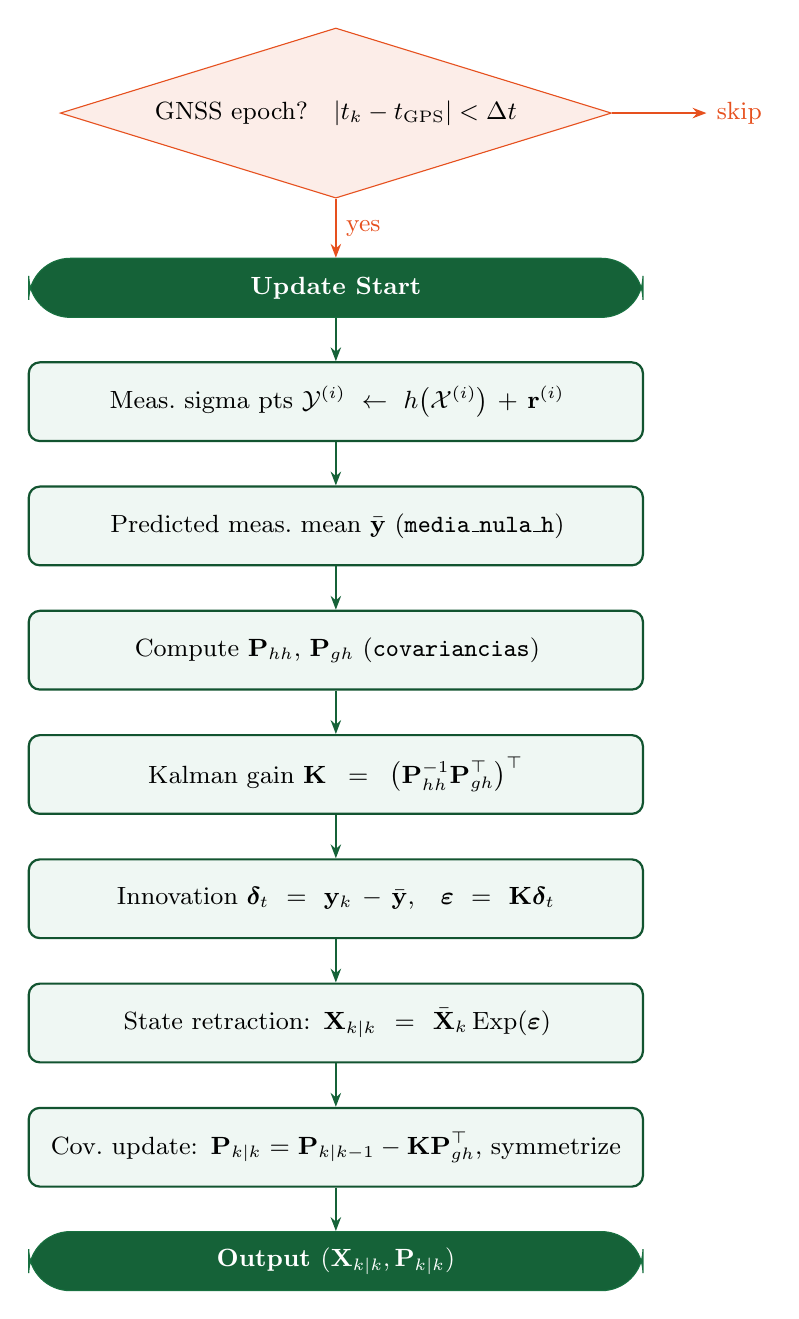
\begin{tikzpicture}[
  node distance=0.55cm,
  start/.style={draw=liegreen!80!black, fill=liegreen!70!black, text=white,
                rounded corners=15pt,
                minimum width=7.8cm, minimum height=0.75cm, font=\small\bfseries},
  flowstep/.style={draw=liegreen!60!black, fill=liegreen!7, rounded corners=4pt,
               minimum width=7.8cm, minimum height=1.0cm,
               text width=7.4cm,
               align=center, font=\small, line width=0.8pt},
  decide/.style={draw=lieaccent, fill=lieaccent!10, diamond, aspect=3.0,
                 minimum width=7cm, align=center, font=\small},
  arr/.style={-{Stealth[length=5pt]}, thick, liegreen!70!black},
  sarr/.style={-{Stealth[length=5pt]}, thick, lieaccent}
]
\node[decide] (check)
  {GNSS epoch?\quad $|t_k-t_{\mathrm{GPS}}|<\Delta t$};
\node[start, below=0.75cm of check] (u0) {Update Start};
\node[flowstep, below=0.55cm of u0] (u1)
  {Meas.\ sigma pts
   $\mathcal{Y}^{(i)}\leftarrow h\bigl(\mathcal{X}^{(i)}\bigr)+\mathbf{r}^{(i)}$};
\node[flowstep, below=0.55cm of u1] (u2)
  {Predicted meas.\ mean $\bar{\mathbf{y}}$
   (\texttt{media\_nula\_h})};
\node[flowstep, below=0.55cm of u2] (u3)
  {Compute $\mathbf{P}_{hh}$, $\mathbf{P}_{gh}$
   (\texttt{covariancias})};
\node[flowstep, below=0.55cm of u3] (u4)
  {Kalman gain
   $\bK=\bigl(\mathbf{P}_{hh}^{-1}\mathbf{P}_{gh}^\top\bigr)^\top$};
\node[flowstep, below=0.55cm of u4] (u5)
  {Innovation $\bm\delta_t=\mathbf{y}_k-\bar{\mathbf{y}}$,\quad
   $\bm\varepsilon=\bK\bm\delta_t$};
\node[flowstep, below=0.55cm of u5] (u6)
  {State retraction:
   $\bX_{k|k}=\bar{\mathbf{X}}_k\,\Exp(\bm\varepsilon)$};
\node[flowstep, below=0.55cm of u6] (u7)
  {Cov.\ update:
   $\bP_{k|k}=\bP_{k|k-1}-\bK\mathbf{P}_{gh}^\top$, symmetrize};
\node[start, below=0.55cm of u7] (u8) {Output $(\bX_{k|k},\bP_{k|k})$};
% yes branch
\draw[sarr] (check) -- node[right, font=\small]{yes} (u0);
% skip branch: go right then down alongside the diagram
\draw[sarr] (check.east) -- ++(1.2,0)
  node[right, font=\small, lieaccent]{skip};
\foreach \a/\b in {u0/u1,u1/u2,u2/u3,u3/u4,u4/u5,u5/u6,u6/u7,u7/u8}
  \draw[arr] (\a) -- (\b);
\end{tikzpicture}
\caption{Update step flowchart.}
\label{fig:upd_flow}
\end{figure}

\subsection{Timing Diagram}

\begin{figure}[h!]
\centering
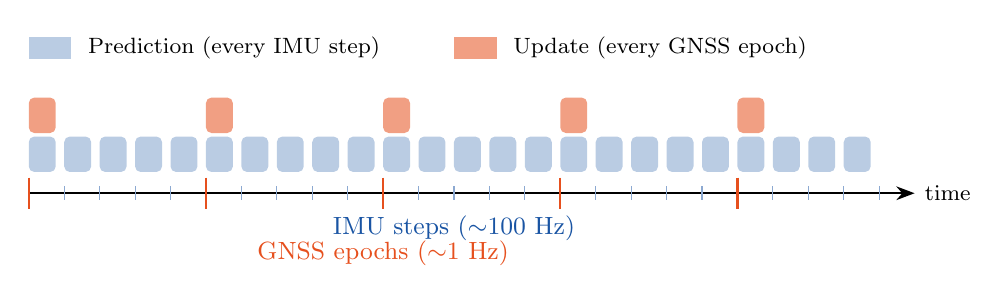
\begin{tikzpicture}[scale=0.9]
\draw[-{Stealth}, thick] (0,0) -- (12.5,0) node[right]{\footnotesize time};
\foreach \x in {0,0.5,...,12}
  \draw[lieblue!50] (\x,0.1) -- (\x,-0.1);
\foreach \x in {0,2.5,5,7.5,10}
  \draw[lieaccent, thick] (\x,0.22) -- (\x,-0.22);
\node[font=\small, lieblue] at (6,-0.5) {IMU steps ($\sim$100 Hz)};
\node[font=\small, lieaccent] at (5,-0.85) {GNSS epochs ($\sim$1 Hz)};
\foreach \x in {0,0.5,1,1.5,2,2.5,3,3.5,4,4.5,5,5.5,6,6.5,7,7.5,8,8.5,9,9.5,10,10.5,11,11.5}
  \fill[lieblue!30, rounded corners=2pt] (\x,0.3) rectangle (\x+0.38,0.8);
\foreach \x in {0,2.5,5,7.5,10}
  \fill[lieaccent!55, rounded corners=2pt] (\x,0.85) rectangle (\x+0.38,1.35);
\fill[lieblue!30] (0,1.9) rectangle (0.6,2.2);
\node[font=\footnotesize, right] at (0.7,2.05) {Prediction (every IMU step)};
\fill[lieaccent!55] (6,1.9) rectangle (6.6,2.2);
\node[font=\footnotesize, right] at (6.7,2.05) {Update (every GNSS epoch)};
\end{tikzpicture}
\caption{Timing of predict/update steps in \texttt{run\_UKF\_Lie.m}.}
\label{fig:timing}
\end{figure}

\subsection{Sigma-Point Geometry}

\begin{figure}[h!]
\centering
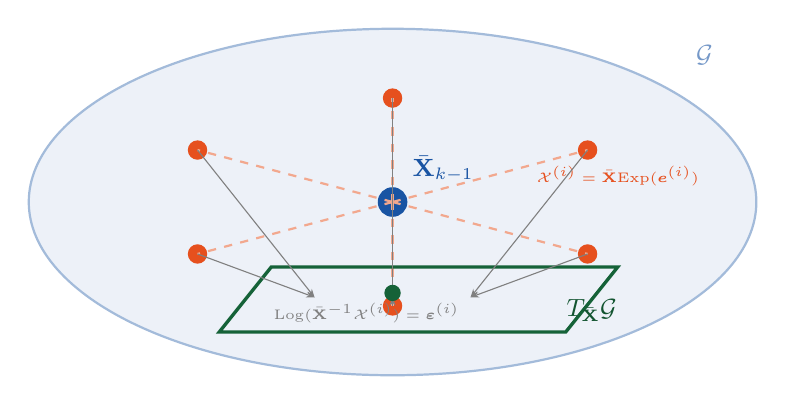
\begin{tikzpicture}[scale=1.1]
\draw[fill=lieblue!8, draw=lieblue!40, thick]
  (0,0) ellipse (4.2cm and 2.0cm);
\node[lieblue!60, font=\small\itshape] at (3.6,1.7) {$\mathcal{G}$};
\filldraw[lieblue, thick] (0,0) circle (4.5pt)
  node[above right=5pt, font=\small\bfseries] {$\bar{\mathbf{X}}_{k-1}$};
\foreach \ang in {30,90,150,210,270,330} {
  \pgfmathsetmacro\px{2.6*cos(\ang)}
  \pgfmathsetmacro\py{1.2*sin(\ang)}
  \filldraw[lieaccent] (\px,\py) circle (3pt);
  \draw[dashed, lieaccent!50, thick] (0,0) -- (\px,\py);
}
\node[font=\tiny, lieaccent] at (2.6,0.3) {$\mathcal{X}^{(i)}=\bar{\mathbf{X}}\Exp(\bm{e}^{(i)})$};
\draw[liegreen!70!black, line width=1.2pt]
  (-2.0,-1.5) -- (2.0,-1.5) -- (2.6,-0.75) -- (-1.4,-0.75) -- cycle;
\node[liegreen!60!black, font=\small\bfseries] at (2.3,-1.25) {$T_{\bar{\mathbf{X}}}\mathcal{G}$};
\foreach \ang in {30,90,150,210,270,330} {
  \pgfmathsetmacro\px{2.6*cos(\ang)}
  \pgfmathsetmacro\py{1.2*sin(\ang)}
  \pgfmathsetmacro\tx{0.4*\px}
  \draw[-{Stealth[length=3pt]}, gray, thin] (\px,\py) -- (\tx,-1.1);
}
\node[gray, font=\tiny\itshape] at (-0.3,-1.28) {$\Log(\bar{\mathbf{X}}^{-1}\mathcal{X}^{(i)})=\bm\varepsilon^{(i)}$};
\filldraw[liegreen!70!black] (0,-1.05) circle (2.5pt);
\end{tikzpicture}
\caption{Sigma points on $\mathcal{G}$ and projection to tangent space $T_{\bar{\mathbf{X}}}\mathcal{G}$ via $\Log$.}
\label{fig:sigpts}
\end{figure}

\section{Implementation Details}

\subsection{Key Functions}

\begin{table}[h!]
\centering
\caption{Key MATLAB functions and their roles.}
\label{tab:functions}
\renewcommand{\arraystretch}{1.35}
\begin{tabular}{@{}llp{5.5cm}@{}}
\toprule
Function & Input/Output & Description \\
\midrule
\texttt{SigmaPointsLie} & $\to(\Xi,W_m,W_c)$ & 67 sigma pts via Cholesky of $\mathbf{P}_\eta$ \\
\texttt{prediction\_UKF\_Lie} & $\to(\bar{\mathbf{X}},\bP,\{\mathcal{X}^{(i)}\},\{\mathbf{r}^{(i)}\})$ & Full prediction \\
\texttt{Update\_UKF\_Lie} & $\to(\bX_{k|k},\bP_{k|k})$ & Full update \\
\texttt{media\_nula\_g} & $\to\bar{\mathbf{X}}$ & Frechet mean on $\mathcal{G}$ \\
\texttt{media\_nula\_h} & $\to\bar{\mathbf{Y}}$ & Mean on $T(3)$ \\
\texttt{covariancias} & $\to(\mathbf{P}_{hh},\mathbf{P}_{gh})$ & Innovation/cross-cov \\
\texttt{exp\_multiSE23T6} & $\mathbb{R}^{15}\to\mathcal{G}$ & Group exponential \\
\texttt{log\_multiSE23T6} & $\mathcal{G}\to\mathbb{R}^{15}$ & Group logarithm \\
\texttt{log\_multiSE3} & $\mathrm{SE}_2(3)\to\mathbb{R}^9$ & Rodrigues-based log \\
\texttt{Omega} & $(\bX,\mathbf{u})\to\mathbb{R}^{15}$ & IMU kinematics \\
\texttt{SingleLlaFromEcef} & $\mathbb{R}^3\to(\lambda,\ell,h)$ & ECEF$\to$geodetic \\
\texttt{gravityModel} & $\lambda\to g$ & WGS-84 gravity \\
\bottomrule
\end{tabular}
\end{table}

\subsection{Initialisation}

\begin{align}
  \bX_0 &= \mathrm{blkdiag}\!\left(
    \begin{pmatrix}\Ceb^0 & \mathbf{0} & \mathbf{p}_0\\\mathbf{0}&\mathbf{I}\end{pmatrix},\,
    \mathbf{I}_4,\,\mathbf{I}_4
  \right)\!, \\
  \bP_0 &= \mathrm{diag}(
    10^{-6}\mathbf{1}_3^\top,\;
    10^{-9}\mathbf{1}_3^\top,\;
    10^{-6}\mathbf{1}_6^\top,\;
    10^{-9}\mathbf{1}_3^\top).
\end{align}

\subsection{Noise Parameters}

\begin{table}[h!]
\centering
\caption{Filter noise standard deviations.}
\renewcommand{\arraystretch}{1.3}
\begin{tabular}{@{}llll@{}}
\toprule
Parameter & Symbol & Value & Units \\
\midrule
Gyroscope & $\sigma_g$ & $10^{-3}$ & rad/s \\
Accelerometer & $\sigma_a$ & $10^{-3}$ & m/s$^2$ \\
Velocity noise & $\sigma_v$ & $10^{-1.5}$ & m/s \\
Gyro bias & $\sigma_{b_g}$ & $10^{-4.5}$ & rad/s \\
Acc. bias & $\sigma_{b_a}$ & $10^{-4.5}$ & m/s$^2$ \\
GNSS position & $\sigma_{\mathrm{GPS}}$ & $10^{-1}$ & m \\
\bottomrule
\end{tabular}
\end{table}

\subsection{Optimisations}

\begin{enumerate}
  \item \textbf{Closed-form $\Log$}: replaced \texttt{eig()} with Rodrigues extraction --- $5$--$10\times$ faster.
  \item \textbf{Geodetic pre-computation}: \texttt{SingleLlaFromEcef} called once/step, not 67 times.
  \item \textbf{LU reuse}: factorize $g$ once per mean iteration, reuse for all sigma-point solves.
  \item \textbf{Cholesky PSD check}: \texttt{chol()} replaces \texttt{eig()} for PD verification.
  \item \textbf{Minor}: pre-transpose \texttt{Cen}, trace via diagonal indexing.
\end{enumerate}

\section{Evaluation}

RMSE metrics:
\[
  \mathrm{RMSE}_p = \sqrt{\frac{1}{N}\sum_k\|\hat{\mathbf{p}}_k-\mathbf{p}_k^{\mathrm{ref}}\|^2},
  \quad
  \mathrm{RMSE}_\psi = \sqrt{\frac{1}{N}\sum_k(\hat\psi_k-\psi_k^{\mathrm{ref}})^2}.
\]

Uncertainty monitor: $\tau_k = \tr(\bP_{k|k})$.

Datasets: \texttt{rectangular}, \texttt{circular}, \texttt{helicoidal}.

\appendix
\section{Code Cross-Reference}

\begin{table}[h!]
\centering
\caption{Equation-to-code mapping.}
\renewcommand{\arraystretch}{1.35}
\begin{tabular}{@{}p{5cm}lp{5cm}@{}}
\toprule
Equation & Section & MATLAB file \\
\midrule
$\Exp$ on $\mathrm{SE}_2(3)$ & 2.2 & \texttt{exp\_multiSE3.m} \\
$\Exp$ on $\mathcal{G}$ & 2.3 & \texttt{exp\_multiSE23T6.m} \\
$\Log$ on $\mathrm{SE}_2(3)$ & 2.2 & \texttt{log\_multiSE3.m} \\
$\Log$ on $\mathcal{G}$ & 2.3 & \texttt{log\_multiSE23T6.m} \\
$\Ad_{\mathbf{X}}$ & 2.3 & \texttt{Ad\_G.m} \\
$[\xi]^\wedge$ bracket & 2.2 & \texttt{bracketUp\_SE\_23.m} \\
$\mathbf{C}_{en}$ & 3.1 & \texttt{DCM\_en.m} \\
$g(\lambda)$ WGS-84 & 3.1 & \texttt{gravityModel.m} \\
ECEF$\to$LLA & 3.1 & \texttt{SingleLlaFromEcef.m} \\
$\Omega(\bX,\mathbf{u})$ & 3.2 & \texttt{Omega.m} \\
Sigma points & 4.2 & \texttt{SigmaPointsLie.m} \\
Propagation & 4.3 & \texttt{prediction\_UKF\_Lie.m} \\
Frechet mean & 4.3 & \texttt{media\_nula\_g.m} \\
$\bP_{k|k-1}$ & 4.3 & \texttt{prediction\_UKF\_Lie.m} \\
Meas. mean & 4.4 & \texttt{media\_nula\_h.m} \\
$\mathbf{P}_{hh},\mathbf{P}_{gh}$ & 4.4 & \texttt{covariancias.m} \\
$\bK$, update & 4.4 & \texttt{Update\_UKF\_Lie.m} \\
Main loop & 5 & \texttt{run\_UKF\_Lie.m} \\
\bottomrule
\end{tabular}
\end{table}

\end{document}
